\subsection{Descripci\'on del problema}

En este ejercicio se nos pide escribir un algoritmo que resuelva una especie de rompecabezas dado por un tablero de $n \times m$ casillas y $n \times m$ fichas.
Cada pieza (cuadrada) tiene un color en cada uno de sus lados, no necesariamente colores distintos en cada uno. Por ejemplo: 

\begin{figure}[h]
\begin{center}
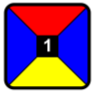
\includegraphics[scale=0.4]{./img/ej3_fichas.png}
\caption{Ejemplo de ficha}
\end{center}
\end{figure}

Ahora, para poder poner una pieza en el tablero debemos asegurarnos de que los colores de los lados coincidan con los de las fichas adyacentes (en caso de que haya una ficha lindante). Un ejemplo de las posicionamiento correcto e incorrecto ser\'ia:\\

\begin{figure}[h]
\begin{center}
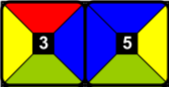
\includegraphics[scale=0.4]{./img/ej3_fichas_coinciden.png}
\caption{Ejemplo posicionamiento correcto}
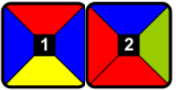
\includegraphics[scale=0.4]{./img/ej3_fichas_ncoinciden.png}
\caption{Ejemplo posicionamiento incorrecto}
\end{center}
\end{figure}

Adem\'as no se pueden girar las piezas por más que esto permita llegar a una mejor soluci\'on.\\
M\'as all\'a de estas restricciones, cualquier pieza puede colocarse en cualquier casillero.\\
La soluci\'on entregada por el algoritmo no necesariamente debe tener el tablero lleno, ya que con el conjunto de piezas dado podr\'ia no existir una forma de ubicarlas todas cumpliendo con lo pedido. Por lo tanto, la soluci\'on al problema debe ser lo m\'as \'optima posible: aquella en la que mayor cantidad de piezas permita ingresar en el tablero dadas las restricciones anteriores.
Por ejemplo el siguiente gr\'afico muestra una soluci\'on \'optima, dado un conjunto de piezas que no permiten llenar por completo el tablero.

\subsection{Resoluci\'on}

Para resolver este problema se nos pidi\'o utilizar la t\'ecnica algor\'itmica de backtracking.\\ 
Comenzamos situados en el primer casillero (superior izquierdo) movi\'endonos de izquierda a derecha y de arriba hacia abajo en el tablero. La idea del algoritmo de backtracking es ir probando, en cada casillero, todas las fichas que pueden ir en esa posici\'on (incluida la pieza en blanco o vac\'ia) y comparar todos los tableros obtenidos qued\'andose con el mejor, es decir, en el que se pudo poner la mayor cantidad de piezas no vac\'ias. \\

La primera optimizaci\'on que realizamos consiste en armar un diccionario de listas que tiene como claves al tipo par($colorIzquierda$, $colorArriba$) y en las listas guarda las fichas que tienen en su lado izquierdo el color $colorIzquierda$ y en su lado superior $colorArriba$. Elegimos esos dos lados por la forma en que recorremos el tablero: al ir de izquierda a derecha y de arriba hacia abajo siempre vamos a tener que hacer coincidir el lado izquierdo de la ficha nuevo con el lado derecho de la que tenga al lado; y el lado superior con el inferior de la que tenga arriba.\\
Vale aclarar que, en caso de tratarse de la primera ficha que ponemos, devolvemos como fichas posibles todo el conjunto dado, ya que no hay ninguna restricci\'on para la primera posici\'on. Lo mismo pasa en caso de que la posici\'on que intentamos llenar no tenga ninguna ficha a la izquierda ni arriba. En caso de que, por ejemplo, s\'olo tenga una ficha arriba con color inferior $colorInf$ pero nada a la izqierda, se devuelven como posibles todas las que tienen $colorInf$ en el lado superior, sin importar lo que tengan en el izquierdo.\\
Contar con ese diccionario nos ahorra tener que probar todas las fichas restantes, reduciendo las posibilidades a s\'olo las que cumplen con esa condici\'on de colores.\\

La segunda optimizaci\'on del algoritmo consiste en crear un tablero de referencia, en el cual iremos guardando el tablero con m\'as fichas (no vac\'ias) puestas obtenido hasta el momento. Inicialmente este tablero tiene cargada una configuraci\'on por defecto, que consiste en poner fichas que no se toquen entre s\'i, que ser\'ia la mejor opci\'on si entre el conjunto dado no hay ning\'un par que coincida.\\

La idea de el tablero de referencia surge a la hora de pensar posibles podas para el \'arbol formado por la recursi\'on del algoritmo de backtranking; ser\'ia innecesario probar todas las combinaciones posibles de fichas (sacadas del diccionario mencionado m\'as arriba) en cada casillero del tablero ya que es  visible que una gran parte de estas no llegar\'ian a ser una soluci\'on \'optima, como puede ser el tablero completamente vac\'io, o el tablero con menos de la mitad de las casillas llenas.

Por lo tanto las podas implementadas son las siguientes:

\begin{itemize}

\item Diccionario de colores: Antes de llamar a la funci\'on backtrack creamos un diccionario con claves par($colorIzq$, $colorArr$) y valores lista($ficha$) donde las fichas cumplen con la condici\'on indicada en la clave. Luego le pasamos este diccionario a backtrack, sac\'andole en cada llamado la ficha usada anteriormente (para que no vuelva a ser usada en el futuro). As\'i nos evitamos tener que probar todas las fichas que quedan y probamos s\'olo las que tiene sentido poner en cada posici\'on.

\item Mejor caso peor que el de referencia: Cada vez que ponemos una ficha hacemos la cuenta de cu\'antas fichas tendr\'ia el tablero actual suponiendo que podamos llenar todas las casillas que faltan recorrer. La cuenta est\'a dada por: $cantidad de fichas puestas$ + $cantidad de posiciones por recorrer$. Si el resultado es menor a la cantidad de fichas puestas en el tablero de referencia, la rama del backtraking que se ocupa de este tablero es podada porque aunque se pudieran colocar fichas en todos los casilleros restantes, no se llegar\'ia a una soluci\'on mejor que la ya obtenida (tablero de referencia). Aqu\'i se regresa al nodo anterior del arbol, cambiando la ficha puesta en este y continuando con el algoritmo.

\item Valor por defecto del tablero de referencia: Antes de comenzar el algoritmo se llena el tablero de referencia en posiciones intercaladas de manera que no importa que fichas coloquemos, al no haber dos fichas juntas cualquier combinaci\'on ser\'a v\'alida. De esta forma obtenemos un tablero con la mitad de los casilleros llenos. Luego, en el caso que las primeras ramas del \'arbol de backtracking resulten menos \'optimas que el tablero de referencia obtenido, no llegaran a completarse, porque se cortaran como resultado de la primer poda.

\item Tablero lleno: Si llegamos a un tablero con todas las fichas puestas (siempre de manera correcta), devolvemos ese tablero y cortamos todas las ramas restantes. En este caso claramente no tiene sentido seguir buscando otras combinaciones, ya que no es posible llegar a una mejor soluci\'on.

\end{itemize}

\subsection{Demostraci\'on de la resoluci\'on}

Para demostrar por qu\'e nuestro algoritmo resuelve el problema de encontrar la soluci\'on \'optima al tablero con las fichas dadas y al tratarse de un algoritmo de backtracking, basta con demostrar por qu\'e con las podas que implementamos no se pierde ning\'un tablero \'optimo.\\

Veamos cada una de las podas:\\

Diccionario de colores. Esta poda nos ahorra probar fichas que no ir\'ian en una posici\'on, dej\'andonos s\'olo las v\'alidas. Es trivial ver que no estamos perdiendo tableros v\'alidos en este caso, ya que las opciones que eliminamos no cumplir\'ian con la condici\'on que pide la consigna.\\

Mejor caso peor que el de referencia. Siendo nuestro tablero de referencia con $m$ fichas puestas, cualquier otro tablero en el que se puedan poner menos fichas nunca llegar\'a a ser \'optimo, con lo cual descartarlo no nos hace perder opciones v\'alidas.\\

Valor por defecto del tablero de referencia. Inicializar el tablero de referencia poniendo las fichas intercaladas es una forma de tener una cota inferior con qu\'e comparar desde el principio de la ejecuci\'on. La explicaci\'on de por qu\'e no nos hace perder opciones es analoga al item anterior, cualquier tablero con fichas intercaladas es v\'alido para todos los tableros posibles. \\

Tablero lleno. Es trivial ver que si encontramos un tablero que cumple con las condiciones pedidas y adem\'as est\'a completo (tiene todas las fichas dadas puestas), no es necesario continuar con la ejecuci\'on del algoritmo ya que no hay tablero m\'as \'optimo que ese.\\

\subsection{Complejidad del algoritmo}

\newpage

\subsection{Codigo fuente}

\lstset{language=C++,
                basicstyle=\ttfamily\footnotesize,
                keywordstyle=\color{blue}\ttfamily,
                stringstyle=\color{red}\ttfamily,
                commentstyle=\color{green}\ttfamily,
                morecomment=[l][\color{magenta}]{\#},
                breaklines=true
}
\begin{lstlisting}

void backtrack(Tablero * tablero, DiccionarioFichas * fichas_ordenadas, Tablero & mejor_tablero) {
	
	list<Ficha> * fichas_posibles;
	
	// Podas
	if(tablero->reject(mejor_tablero)){ 
		return; 
	}
	
	// Si encuentro un tablero completo termino, si es un tablero mejor que el mejor actual lo reemplazo
	if(tablero->accept(mejor_tablero)){ 
		return; 
	}
	
	if(tablero->getPosicionesRecorridas() < (tablero->getFilas() * tablero->getColumnas())){
				
		// Solo recorro las fichas que pueden ir en ese lugar, osea, las que coinciden el color superior e izquierdo con la ficha de arriba y la de atras
		// Si es la 1ra posicion o no tengo fichas arriba o atras, puedo poner todas
		pair<Color, Color> restriccion = tablero->restriccionFicha(tablero->getPosicionLibre());
		fichas_posibles = fichas_ordenadas->dameFichas(restriccion);
		

		// Recorro las fichas que vale la pena ubicar
		for(list<Ficha>::iterator f = fichas_posibles->begin(); f != fichas_posibles->end(); f++){

			// Para cada ficha restante, llamo un backtracking con el tablero
			// y agrego la proxima ficha al nuevo tablero
			Tablero* tablero_con_una = new Tablero(*tablero);
			tablero_con_una->agregarFicha(*f);

			// Le paso al proximo bt las fichas sin la que puse para no repetir
			DiccionarioFichas * fichas_ordenadas_sin_una = new DiccionarioFichas(*fichas_ordenadas);
			fichas_ordenadas_sin_una->sacarFicha(*f);	

			backtrack(tablero_con_una, fichas_ordenadas_sin_una, mejor_tablero);

			delete tablero_con_una;
			delete fichas_ordenadas_sin_una;
		}
		
		// Limpio las fichas temporales
		delete fichas_posibles;
		
		// Siempre considero el caso de no agregar ficha
		Tablero* tablero_con_vacia = new Tablero(*tablero);
		Ficha fvacia = Ficha();
		tablero_con_vacia->agregarFicha(fvacia);
			
		backtrack(tablero_con_vacia, fichas_ordenadas, mejor_tablero);
		
		delete tablero_con_vacia;
	
	}
	
}

\end{lstlisting}

\newpage

\subsection{Casos de prueba}

\subsection{Performance}
